\documentclass[a4paper,12pt]{jarticle}
\usepackage[dvipdfmx]{graphicx}
\usepackage{amsmath}
\usepackage{subfigure}
\usepackage{comment}
\usepackage{listings}

\setlength{\hoffset}{0cm}
\setlength{\oddsidemargin}{-3mm}
\setlength{\evensidemargin}{-3cm}
\setlength{\marginparsep}{0cm}
\setlength{\marginparwidth}{0cm}
\setlength{\textheight}{24.7cm}
\setlength{\textwidth}{17cm}
\setlength{\topmargin}{-45pt}

\renewcommand{\baselinestretch}{1.6}
\renewcommand{\floatpagefraction}{1}
\renewcommand{\topfraction}{1}
\renewcommand{\bottomfraction}{1}
\renewcommand{\textfraction}{0}
\renewcommand{\labelenumi}{(\arabic{enumi})}
%\renewcommand{\figurename}{Fig.} %図をFig.にする


%図のキャプションからコロン:を消す
\makeatletter
\long\def\@makecaption#1#2{% #1=図表番号、#2=キャプション本文
\sbox\@tempboxa{#1. #2}
\ifdim \wd\@tempboxa >\hsize
#1 #2\par 
\else
\hb@xt@\hsize{\hfil\box\@tempboxa\hfil}
\fi}
\makeatother
% 

%Listingnameの定義
\def\lstlistingname{Program}
%
\title{車両制御特論 \\
レポート2\\
}
\author{\vspace{40mm}\\
九州工業大学大学院 \hspace{0mm} 工学府\\
機械知能工学専攻\ \hspace{0mm} 知能制御工学コース \\
\vspace{5mm}\\
所属:\ 西田研究室\\
学籍番号:\ 16344217\\
提出者氏名:\ 津上 \hspace{0mm} 祐典\\\vspace{5mm}\\ }
\date{平成28年\ 8月\ 10日}

\begin{document}

%表紙
\titlepage
\maketitle
\thispagestyle{empty}

\newpage
%%%%%%%%%%%%%%%%%%%%%%%%%%%
\section{与えられたシステム}
%%%%%%%%%%%%%%%%%%%%%%%%%%%
学籍番号によって決まった制御対象は,
\begin{equation}
 \dot{x}(t) = ax^3(t) + b \cos 2t + c(x^2(t)+1)u(t) \\
\end{equation}
%
\begin{equation}
 a = 3 ,\ b = -6 , \ c = 2 
\end{equation}
%
である.また,理想モデルは,
\begin{equation}\label{equ:ideal_model}
 \dot{x}_d(t) = -4x_d(t)+r_d(t)
\end{equation}
である.ここで,
\begin{equation}
 \tilde{x}(t) = x(t) - x_d(t) 
\end{equation}
とおくと追従誤差方程式は,
\begin{eqnarray}
 \dot{\tilde{x}}(t) & = & \dot{x}(t) - \dot{x}_d(t) \\
 & = & ax^3(t) + b \cos 2t + c(x^2(t)+1)u(t) - \dot{x}_d(t)
\end{eqnarray}
となる.
%
%%%%%%%%%%%%%%%%%%%%%%%%%%%
\section{適応追従コントローラの設計}
%%%%%%%%%%%%%%%%%%%%%%%%%%%

%%%%%%%%%%%%%%%%%%%%%%%%%%%%%
\subsection{$a,b,c$が既知のとき}
%%%%%%%%%%%%%%%%%%%%%%%%%%%%
エネルギー関数を$V(t)=\tilde{x}^2(t)$とおく.エネルギー関数の時間微分を
解析すると,
%
\begin{eqnarray}
 \dot{V}(t) & = & 2\tilde{x}(t)\dot{\tilde{x}}(t) \\ 
  & = & 2\tilde{x}(t) \biggl[ax^3(t) + b \cos 2t+c\bigl\{x^2(t)+1 \bigr\}u(t)-\dot{x}_d(t)\biggr] 
\end{eqnarray}
%
となる.ここで入力$u(t)$を
\begin{equation}
 u(t) = -\frac{ax^3(t)}{c(x^2(t)+1)} -\frac{b \cos 2t}{c(x^2(t)+1)}
  +\frac{\dot{x}_d(t)}{c(x^2(t)+1)} - \delta \tilde{x}(t) \ \ \ \ (\delta > 0)
\end{equation}
%
とすれば,
%
\begin{equation}
 \dot{V}(t) = -2\delta c (x^2(t)+1)\tilde{x}^2(t) < 0 \ \ \ \ \ \ for \ any \ \tilde{x}(t)\neq 0
\end{equation}
となり,システムを漸近安定化することが出来る.
%%%%%%%%%%%%%%%%%%%%%%%%%%%%%
\subsection{$a,b,c$が未知のとき}
%%%%%%%%%%%%%%%%%%%%%%%%%%%%
次に,$a,b,c$が未知な場合を考える.入力$u(t)$を
\begin{eqnarray}
 u(t)& = & -\frac{\hat{a}}{\hat{c}}\frac{x^3(t)}{x^2(t)+1} -\frac{\hat{b}}{\hat{c}}\frac{\cos 2t}{x^2(t)+1}
  +\frac{1}{\hat{c}}\frac{\dot{x}_d(t)}{x^2(t)+1} - \delta \tilde{x}(t) \\
  & = & -\hat{\alpha}\frac{x^3(t)}{x^2(t)+1} +\hat{\beta}\frac{\cos 2t}{x^2(t)+1}
  +\hat{\gamma}\frac{\dot{x}_d(t)}{x^2(t)+1} - \delta \tilde{x}(t)
\end{eqnarray}
%
とすると,誤差追従方程式は,
%
\begin{eqnarray}
 \dot{\tilde{x}}(t)& =& ax^3(t) + b \cos 2t - \dot{x}_d(t) -c\hat{\alpha}x^3(t) -c\hat{\beta}\cos 2t
  +c\hat{\gamma}\dot{x}_d(t) - c\delta \bigl\{x^2(t) + 1 \bigr\}
 \tilde{x}(t)\\
 &=&c\tilde{\alpha}x^3(t) +c\tilde{\beta}\cos 2t
  -c\tilde{\gamma}\dot{x}_d(t) - c\delta \bigl\{x^2(t)+1 \bigr\}\tilde{x}(t)
\end{eqnarray}
となる.ただし,
$\tilde{\alpha}=\alpha-\hat{\alpha},\tilde{\beta}=\beta-\hat{\beta},\tilde{\gamma}=\gamma-\hat{\gamma}$
である.エネルギー関数を
\begin{equation}
 V(t) = \tilde{x}^2(t) + \eta^{-1}_{\alpha}c\tilde{\alpha}^2+\eta^{-1}_{\beta}c\tilde{\beta}^2+\eta^{-1}_{\gamma}c\tilde{\gamma}^2
\end{equation}
とおく.ただし,
$\eta_{\alpha},\eta_{\beta},\eta_{\gamma}$は推定ゲインで
ある.次に,エネルギー関数の時間微分を解析すると,
%
\begin{equation}
\dot{V}(t) =  2\tilde{x}(t)\dot{\tilde{x}}(t) +
 2\eta^{-1}_{\alpha}c\tilde{\alpha}\dot{\tilde{\alpha}}
 +2\eta^{-1}_{\beta}c\tilde{\beta}\dot{\tilde{\beta}} +
 2\eta^{-1}_{\gamma}c\tilde{\gamma}\dot{\tilde{\gamma}}
\end{equation}
%
より
\begin{multline}
   \dot{V}(t)= 2\tilde{x}(t)\bigl[ c\tilde{\alpha}x^3(t) +c\tilde{\beta}\cos 2t
  -c\tilde{\gamma}\dot{x}_d(t) - c\delta \bigl\{x^2(t)+1\bigr\}
 \tilde{x}(t)\bigr]\\ 
 + 2\eta^{-1}_{\alpha}c\tilde{\alpha}\dot{\tilde{\alpha}}
 +2\eta^{-1}_{\beta}c\tilde{\beta}\dot{\tilde{\beta}} +
  2\eta^{-1}_{\gamma}c\tilde{\gamma}\dot{\tilde{\gamma}} 
\end{multline}
%
となる.ここで,
\begin{eqnarray}
\dot{\tilde{\alpha}}&=&-\dot{\hat{\alpha}}=-\eta_{\alpha}\tilde{x}(t)x^3(t) \\
\dot{\tilde{\beta}}&=&-\dot{\hat{\beta}}=-\eta_{\beta}\tilde{x}(t) \cos 2t\\
\dot{\tilde{\gamma}}&=&-\dot{\hat{\gamma}}=\eta_{\gamma}\tilde{x}(t)\dot{x}_d(t)   
\end{eqnarray}
とすれば,
%
\begin{equation}
\dot{V}(t) = -2\delta c (x^2(t)+1)\tilde{x}^2(t) \leq 0 \ \ \ \ \ \ for \ any \ \ \begin{pmatrix}
\tilde{x}(t)\\ \tilde{\alpha}\\ \tilde{\beta}\\ \tilde{\gamma}\\
\end{pmatrix}
\neq
\begin{pmatrix}
0\\ 0\\ 0\\ 0\\ 
\end{pmatrix}								
\end{equation}
%
となり,システムを安定化出来る.

以上より,以下の適応追従コントローラを得る.

\begin{eqnarray}
  u(t)&=& -\hat{\alpha}\frac{x^3(t)}{x^2(t)+1} +\hat{\beta}\frac{\cos 2t}{x^2(t)+1}
  +\hat{\gamma}\frac{\dot{x}_d(t)}{x^2(t)+1} - \delta \tilde{x}(t) \\
  \dot{\hat{\theta}}(t)
  &=&
  \begin{pmatrix}
	 \dot{\hat{\alpha}}\\ \dot{\hat{\beta}}\\ \dot{\hat{\gamma}}\\
  \end{pmatrix}
  =
  \begin{pmatrix}
   \eta_{\alpha}\tilde{x}(t)x^3(t)\\
   \eta_{\beta}\tilde{x}(t)\cos 2t\\
   -\eta_{\gamma}\tilde{x}(t)\dot{x}_d(t)\\
  \end{pmatrix}
\end{eqnarray}

%%%%%%%%%%%%%%%%%%%%%%%%%%%%%
\section{シミュレーション}
%%%%%%%%%%%%%%%%%%%%%%%%%%%%
Simulinkで構成したモデルを以下にそれぞれ示す.システムの全体
を図\ref{fig:zentai}に,理想モデルを図\ref{fig:ideal}に,制御対象を図\ref{fig:System}に,制御入力を図
\ref{fig:input}に示す.
また,図\ref{fig:alpha} - \ref{fig:gamma}に$\alpha,\beta,\gamma$の推定器を
示し,図\ref{fig:delta}に$\delta$に関するサブシステムを示す.
%
\begin{figure}[b]
    \begin{center}
       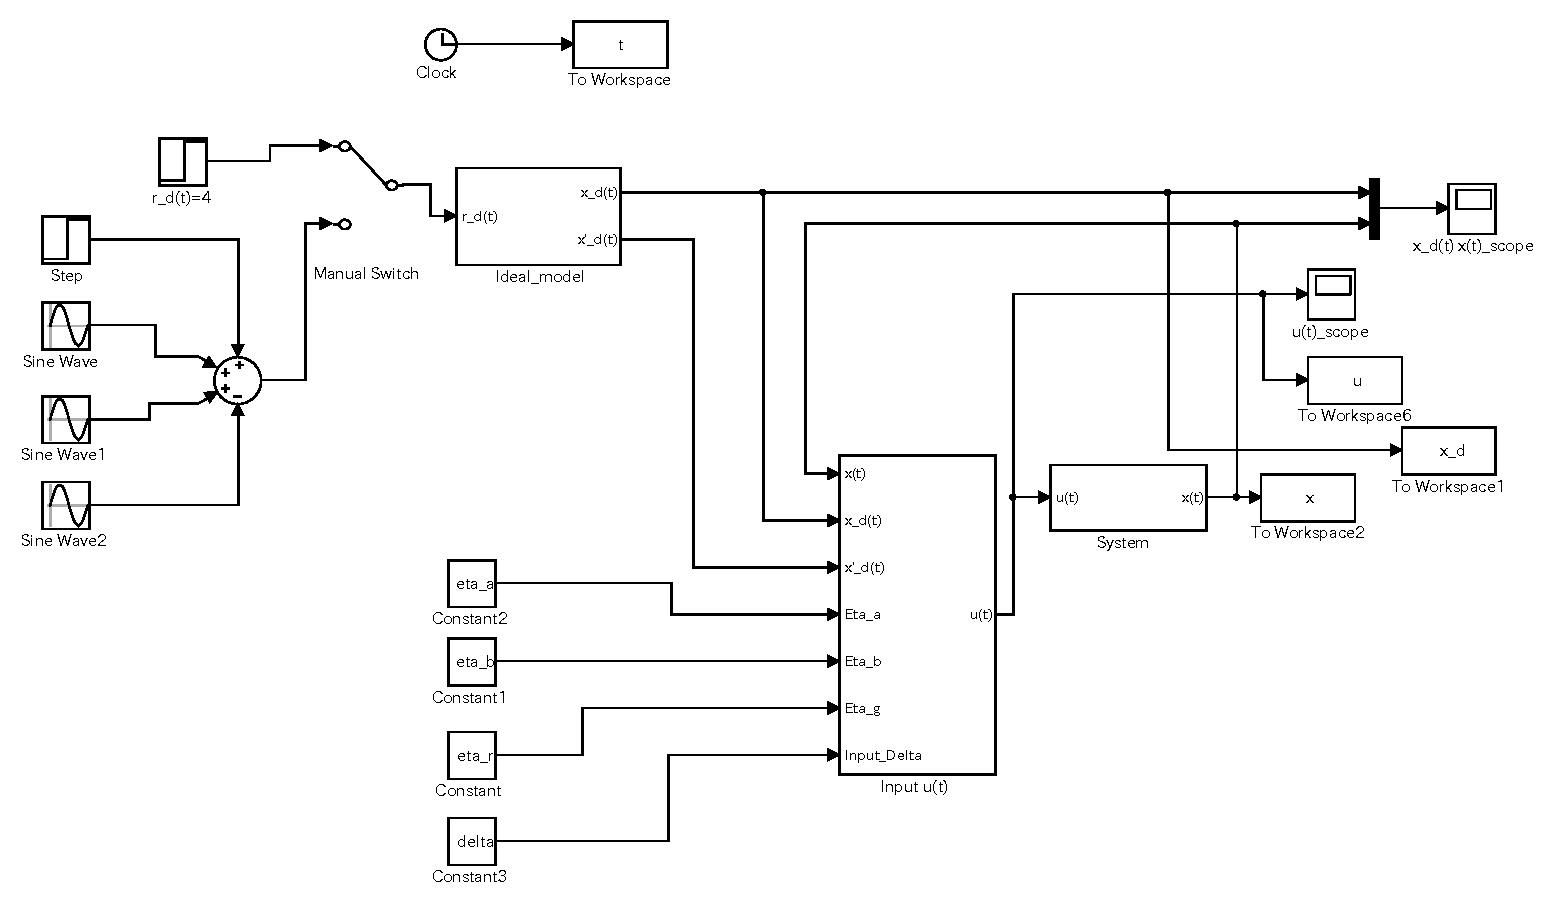
\includegraphics[width=170mm]{fig/zentai.eps}
        \caption{構成したモデルの全体図}
        \label{fig:zentai}
    \end{center}
 \end{figure}
%
%
\begin{figure}[tb]
    \begin{center}
       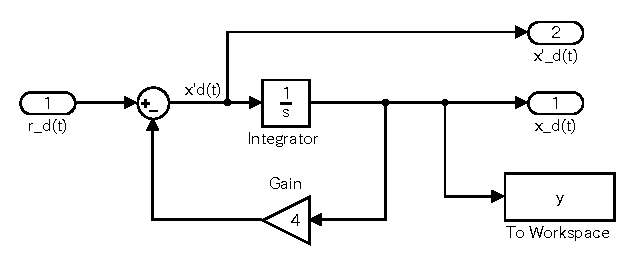
\includegraphics[width=100mm]{fig/ideal.eps}
        \caption{理想モデル}
        \label{fig:ideal}
    \end{center}
 \end{figure}
 %
 %
\begin{figure}[tb]
    \begin{center}
       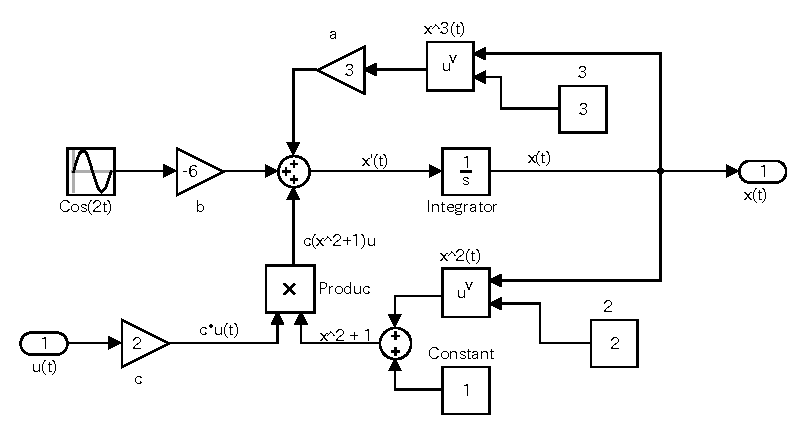
\includegraphics[width=120mm]{fig/System.eps}
        \caption{制御対象}
        \label{fig:System}
    \end{center}
 \end{figure}
%
%
\begin{figure}[tb]
    \begin{center}
       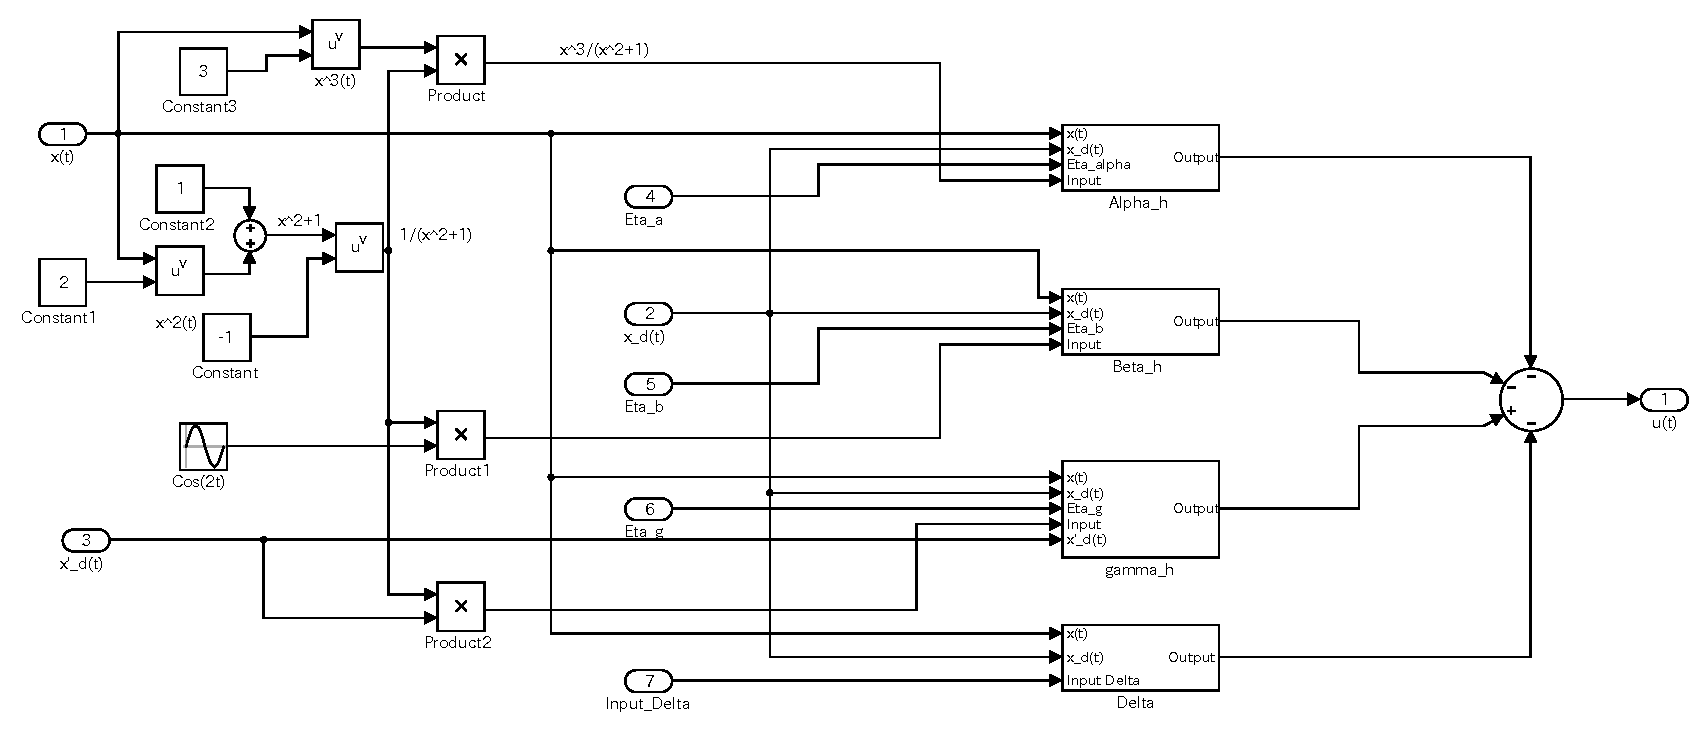
\includegraphics[width=170mm]{fig/input.eps}
        \caption{入力$u(t)$}
        \label{fig:input}
    \end{center}
 \end{figure}
 %
 %
\begin{figure}[htb]
    \begin{center}
       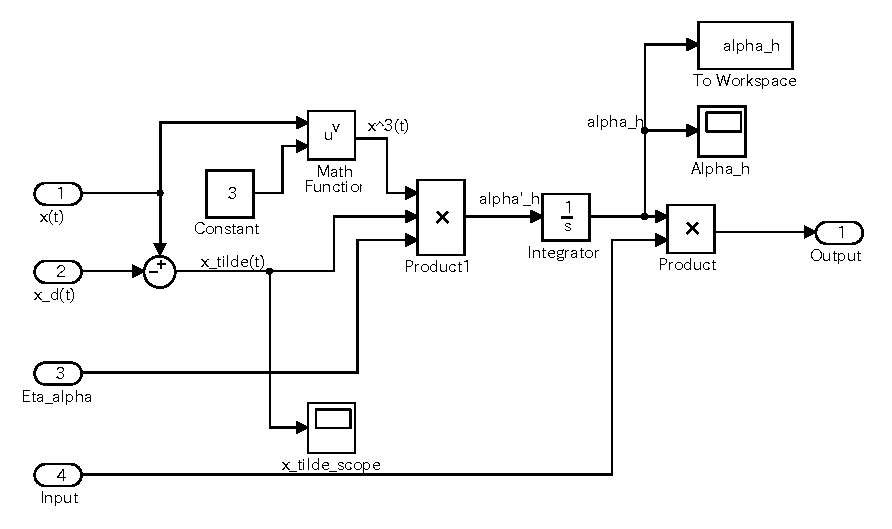
\includegraphics[width=105mm]{fig/alpha.eps}
        \caption{$\hat{\alpha}$の推定器}
        \label{fig:alpha}
    \end{center}
 \end{figure}
 %
%
\begin{figure}[htb]
    \begin{center}
       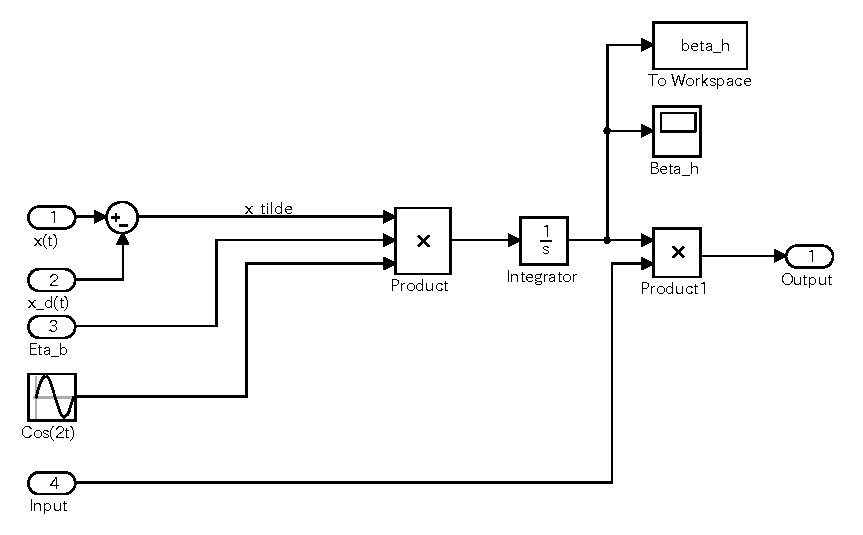
\includegraphics[width=105mm]{fig/beta.eps}
        \caption{$\hat{\beta}$の推定器}
        \label{fig:beta}
    \end{center}
 \end{figure}
%
%
\begin{figure}[htb]
    \begin{center}
       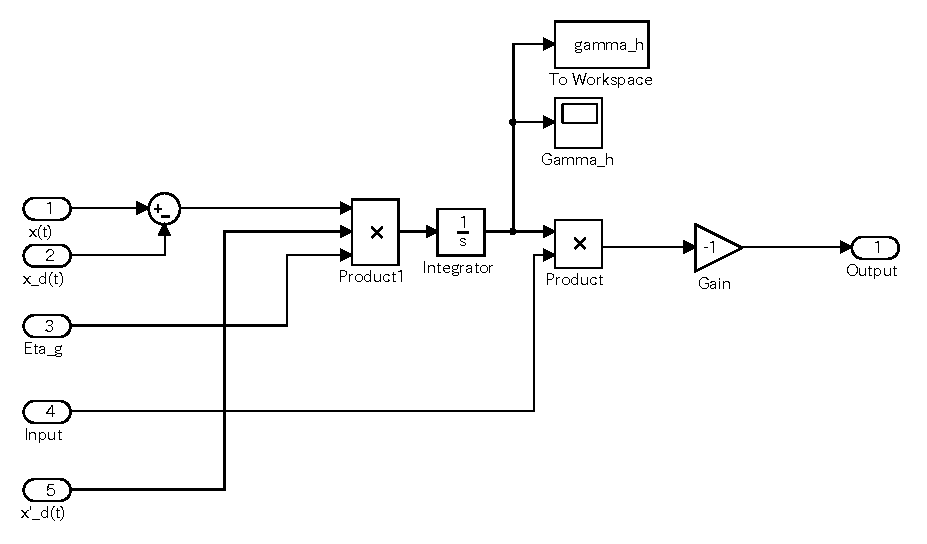
\includegraphics[width=105mm]{fig/gamma.eps}
        \caption{$\hat{\gamma}$の推定器}
        \label{fig:gamma}
    \end{center}
 \end{figure}
%
%
\begin{figure}[htb]
    \begin{center}
       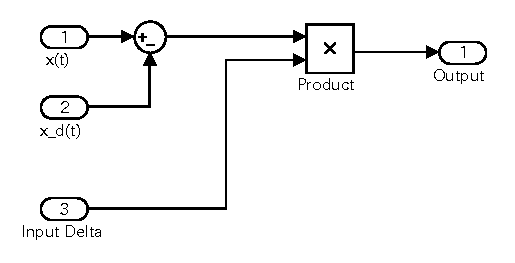
\includegraphics[width=70mm]{fig/delta.eps}
        \caption{$\delta$に関するサブシステム}
        \label{fig:delta}
    \end{center}
 \end{figure}
 %
%%%%%%%%%%%%%%%%%%%%%%%%%%%%%
\subsection{$r_d(t)=4$の場合}
%%%%%%%%%%%%%%%%%%%%%%%%%%%%
(\ref{equ:ideal_model})式にて$r_d(t)=4$とした場合,シミュレーションし
た結果を図\ref{fig:x_rd4}示す.また,図\ref{fig:x_tilde_rd4}に追従誤差
$\tilde{x}(t)$,図\ref{fig:u_rd4}に入力$u(t)$を,図\ref{fig:alpha_h_rd4}
- \ref{fig:gamma_h_rd4}に
$\hat{\alpha},\hat{\beta},\hat{\gamma}$を示す.ただし,$\eta_\alpha=\eta_\beta=\eta_\gamma=1$とした.
%
\begin{figure}[htb]
    \begin{center}
       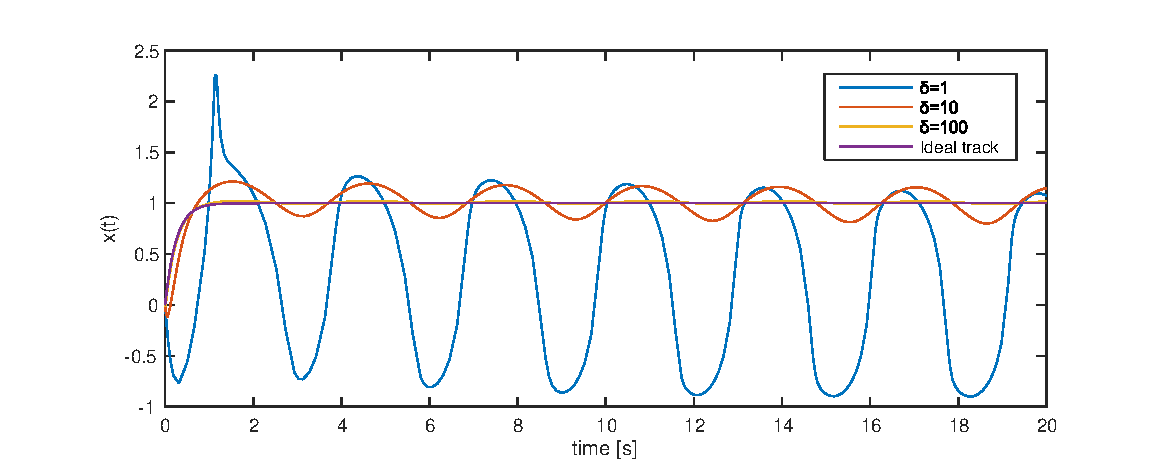
\includegraphics[width=140mm]{fig/x_rd4.eps}
        \caption{$r_d(t)=4$のときの理想軌道と$x$($\delta=1,10,100$)の比較}
        \label{fig:x_rd4}
    \end{center}
\end{figure}
%
%
\begin{figure}[tb]
    \begin{center}
       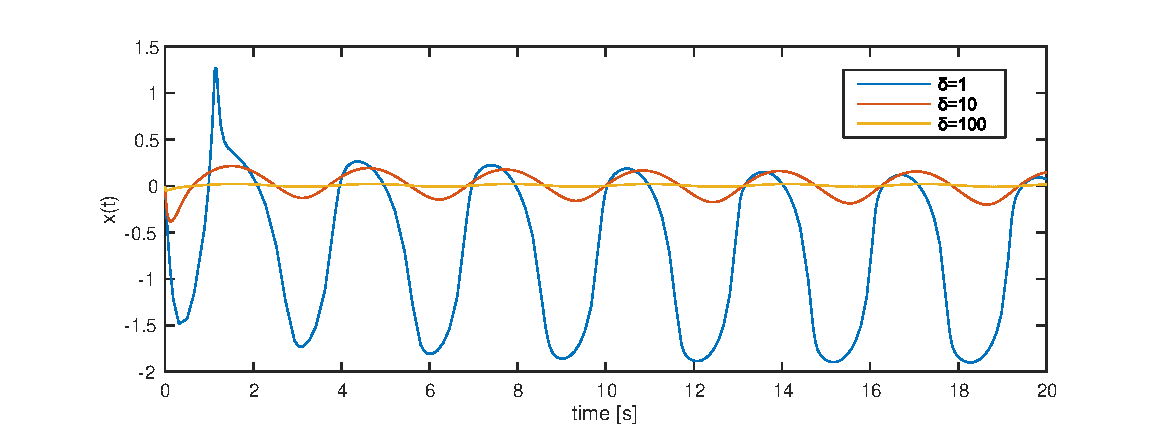
\includegraphics[width=140mm]{fig/x_tilde_rd4.eps}
        \caption{$r_d(t)=4$のときの$\tilde{x}$($\delta=1,10,100$)の様
	 子}
        \label{fig:x_tilde_rd4}
    \end{center}
\end{figure}
%
%
\begin{figure}[htb]
    \begin{center}
       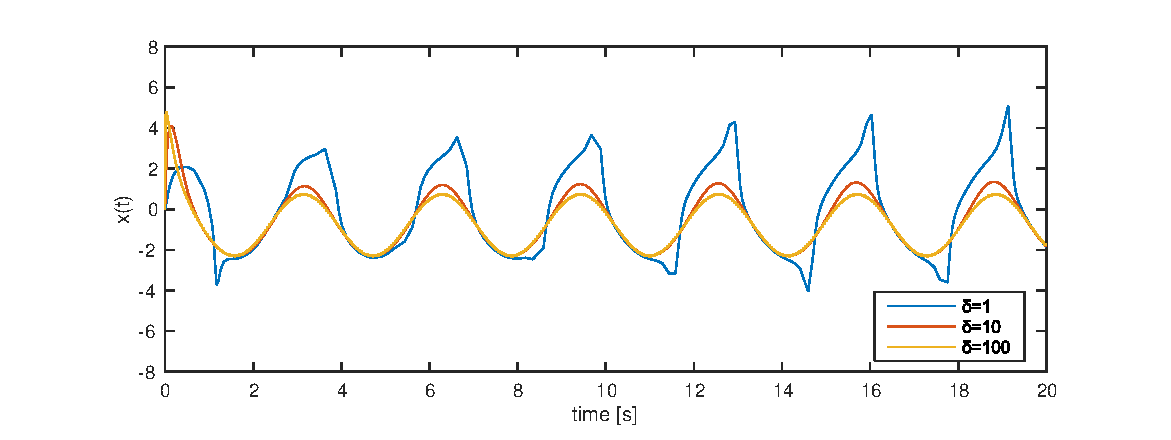
\includegraphics[width=140mm]{fig/u_rd4.eps}
        \caption{$r_d(t)=4$のときの$u(t)$($\delta=1,10,100$)の様子}
        \label{fig:u_rd4}
    \end{center}
\end{figure}
%
\begin{figure}[htb]
    \begin{center}
       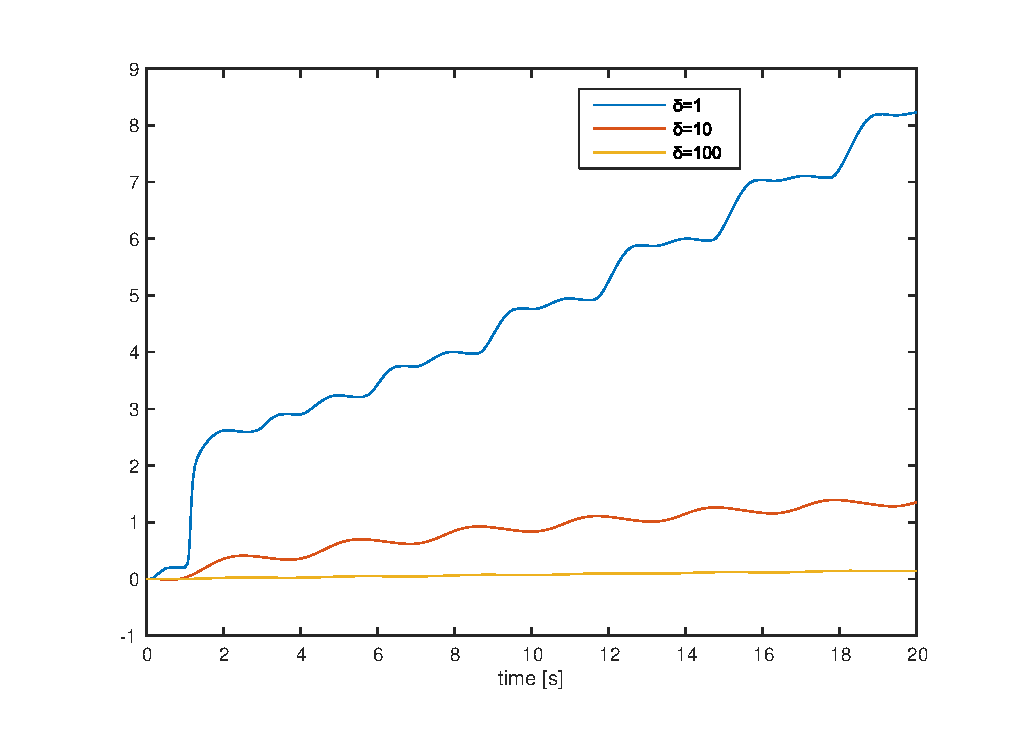
\includegraphics[width=95mm]{fig/alpha_h_rd4.eps}
        \caption{$r_d(t)=4$のときの$\hat{\alpha}$($\delta=1,10,100$)の様子}
        \label{fig:alpha_h_rd4}
    \end{center}
\end{figure}
%
%
\begin{figure}[htb]
    \begin{center}
       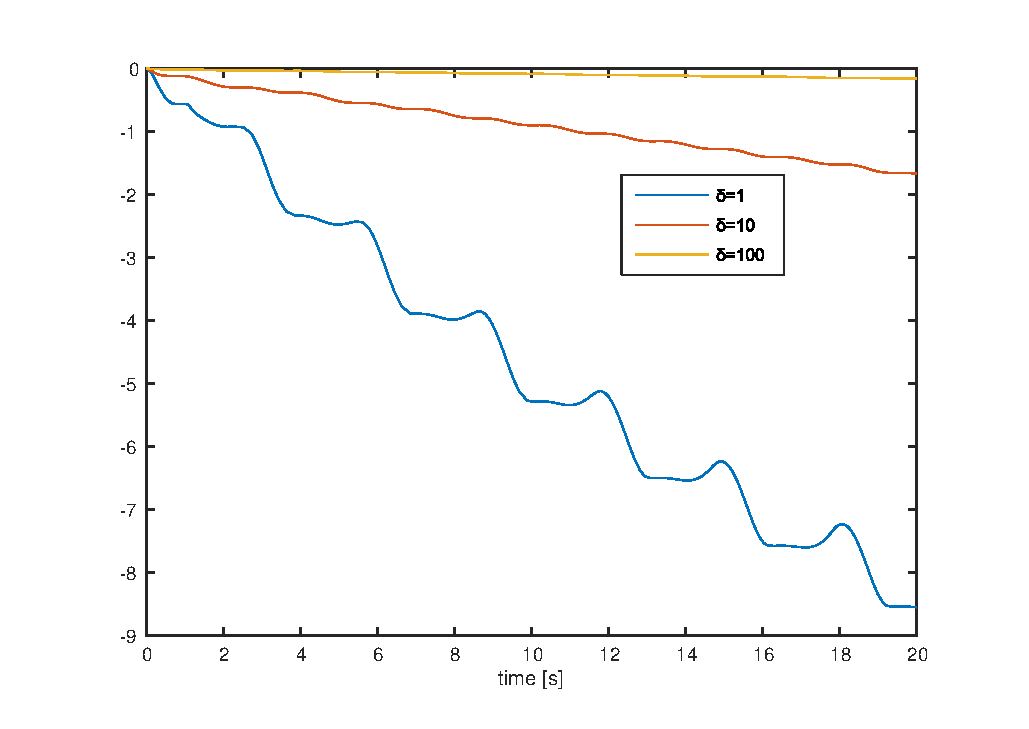
\includegraphics[width=95mm]{fig/beta_h_rd4.eps}
        \caption{$r_d(t)=4$のときの$\hat{\beta}$($\delta=1,10,100$)の様子}
        \label{fig:beta_h_rd4}
    \end{center}
\end{figure}
%
%
\begin{figure}[htb]
    \begin{center}
       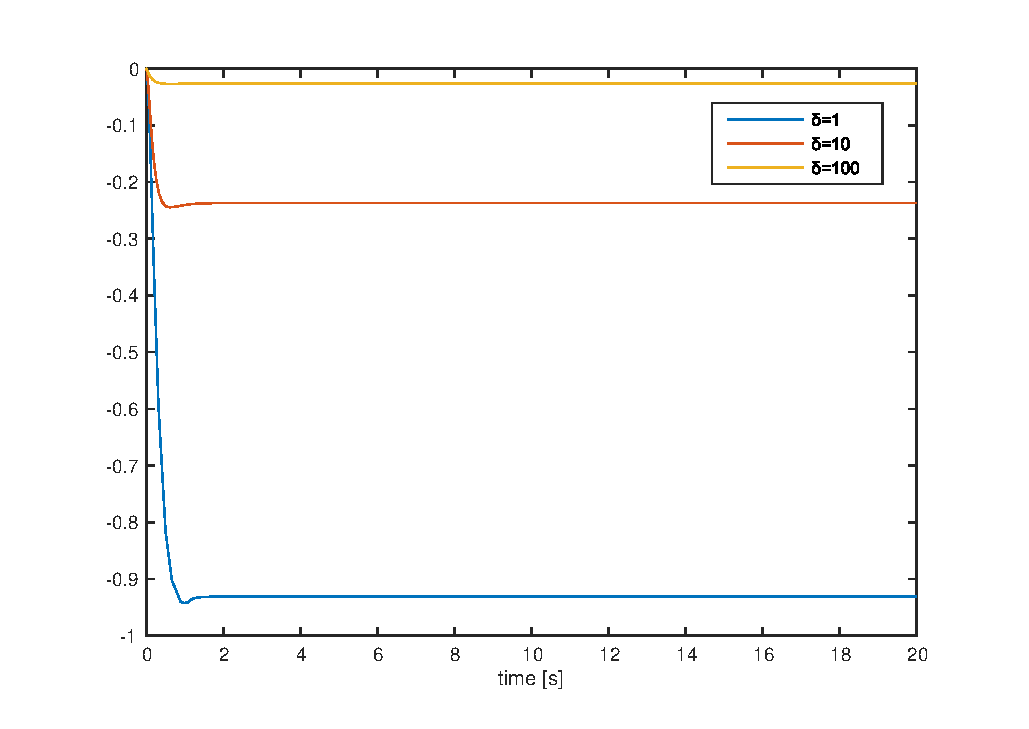
\includegraphics[width=95mm]{fig/gamma_h_rd4.eps}
        \caption{$r_d(t)=4$のときの$\hat{\gamma}$($\delta=1,10,100$)の様子}
        \label{fig:gamma_h_rd4}
    \end{center}
\end{figure}
%

%%%%%%%%%%%%%%%%%%%%%%%%%%%%%
\subsection{$r_d(t)=4+0.5\sin 0.5t + \cos 3t - 2\sin 5t$の場合}
%%%%%%%%%%%%%%%%%%%%%%%%%%%%
$r_d(t)=4$の場合と同様にシミュレーションした結果を図\ref{fig:x_rdsin}
- \ref{fig:gamma_h_rdsin}にそれぞれ示す.
%
\begin{figure}[htb]
    \begin{center}
       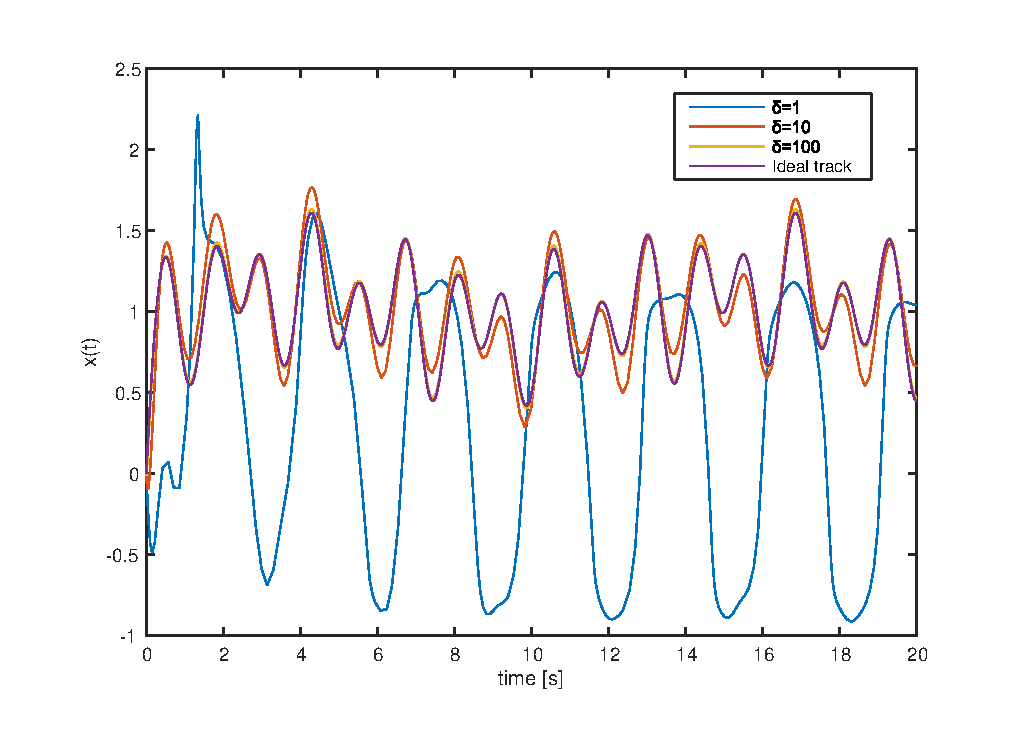
\includegraphics[width=140mm]{fig/x_rdsin.eps}
        \caption{$r_d(t)=4+0.5\sin 0.5t + \cos 3t - 2\sin 5t$のときの理想軌道と$x$($\delta=1,10,100$)の比較}
        \label{fig:x_rdsin}
    \end{center}
\end{figure}
%
%
\begin{figure}[htb]
    \begin{center}
       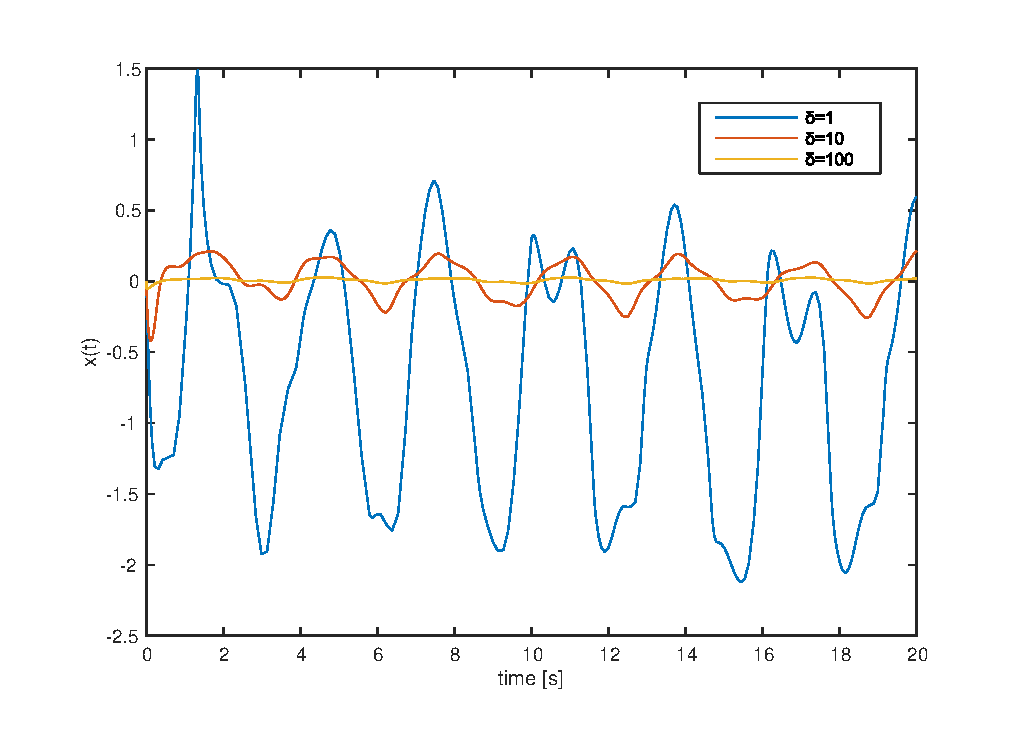
\includegraphics[width=140mm]{fig/x_tilde_rdsin.eps}
        \caption{$r_d(t)=4+0.5\sin 0.5t + \cos 3t - 2\sin 5t$のときの$\tilde{x}$($\delta=1,10,100$)の様子}
        \label{fig:x_tilde_rdsin}
    \end{center}
\end{figure}
%
%
\begin{figure}[htb]
    \begin{center}
       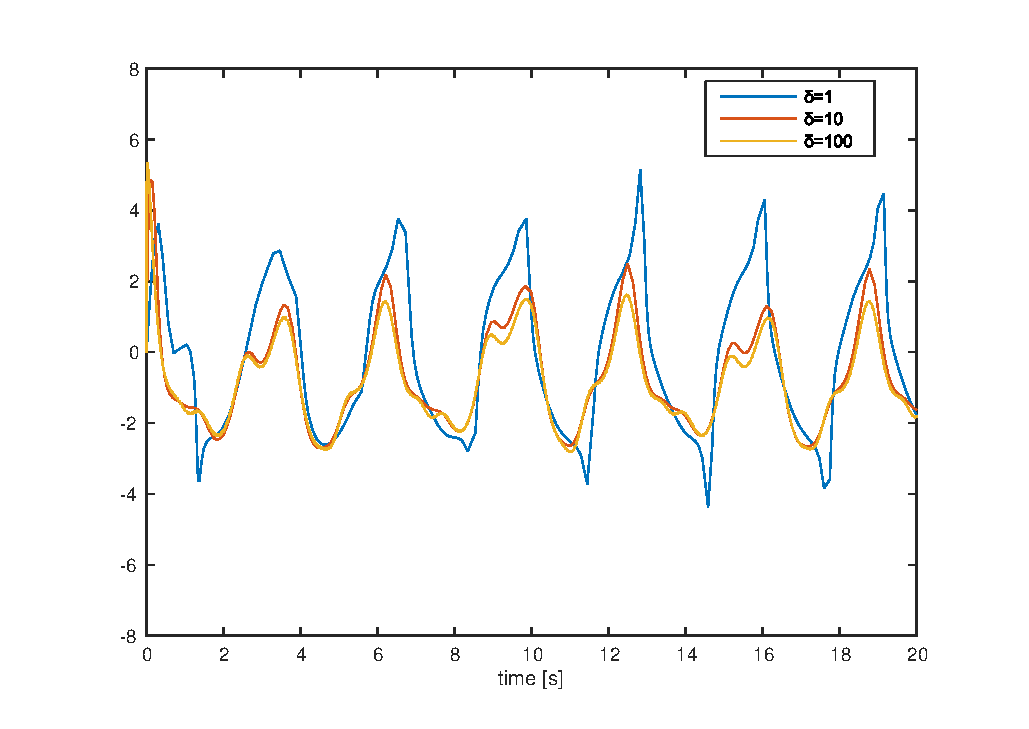
\includegraphics[width=140mm]{fig/u_rdsin.eps}
        \caption{$r_d(t)=4+0.5\sin 0.5t + \cos 3t - 2\sin 5t$のときの$u(t)$($\delta=1,10,100$)の様子}
        \label{fig:u_rdsin}
    \end{center}
\end{figure}
%
%
\begin{figure}[htb]
    \begin{center}
       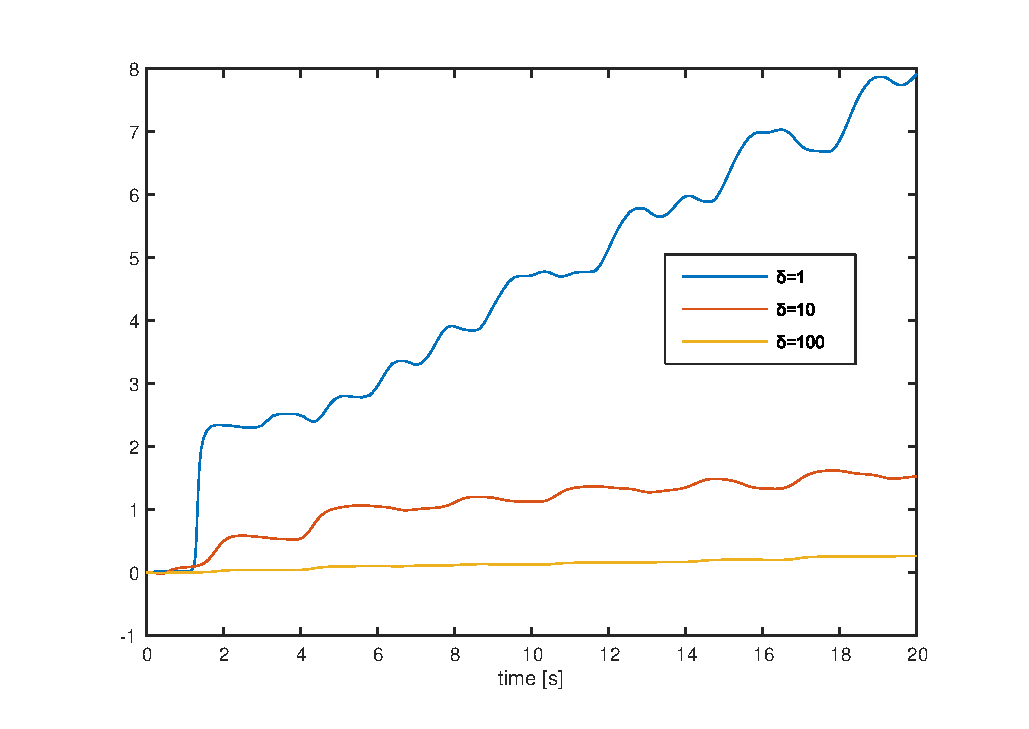
\includegraphics[width=85mm]{fig/alpha_h_rdsin.eps}
        \caption{$r_d(t)=4+0.5\sin 0.5t + \cos 3t - 2\sin 5t$のときの$\hat{\alpha}$($\delta=1,10,100$)の様子}
        \label{fig:alpha_h_rdsin}
    \end{center}
\end{figure}
%
%
\begin{figure}[htb]
    \begin{center}
       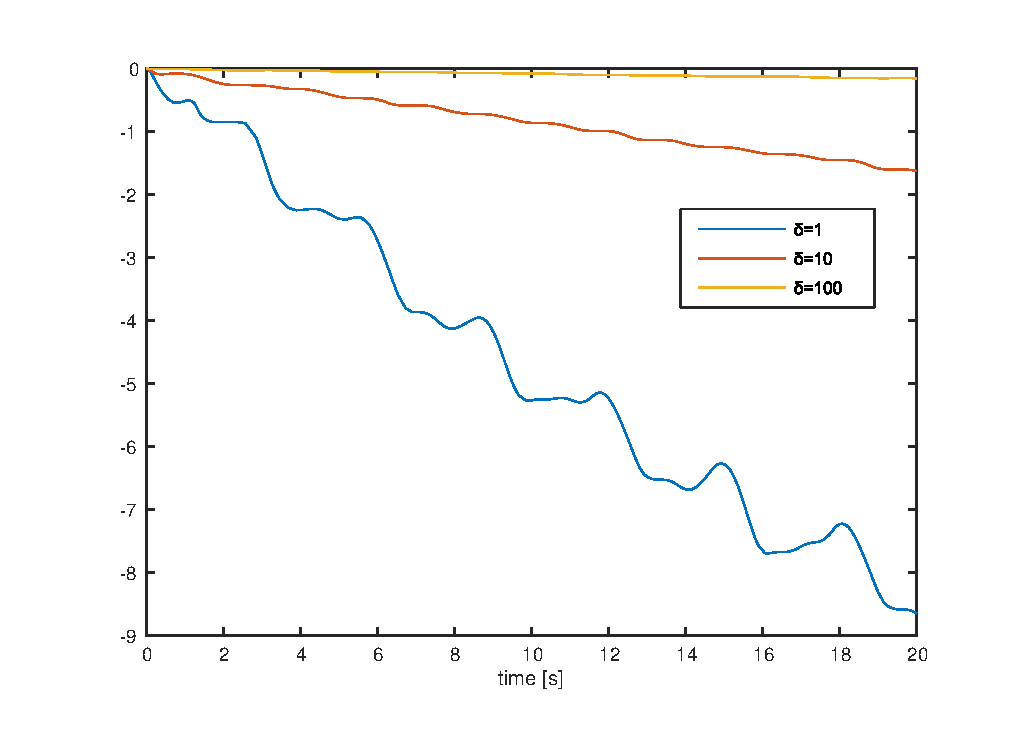
\includegraphics[width=85mm]{fig/beta_h_rdsin.eps}
        \caption{$r_d(t)=4+0.5\sin 0.5t + \cos 3t - 2\sin 5t$のときの$\hat{\beta}$($\delta=1,10,100$)の様子}
        \label{fig:beta_h_rdsin}
    \end{center}
\end{figure}
%
%
\begin{figure}[htb]
    \begin{center}
       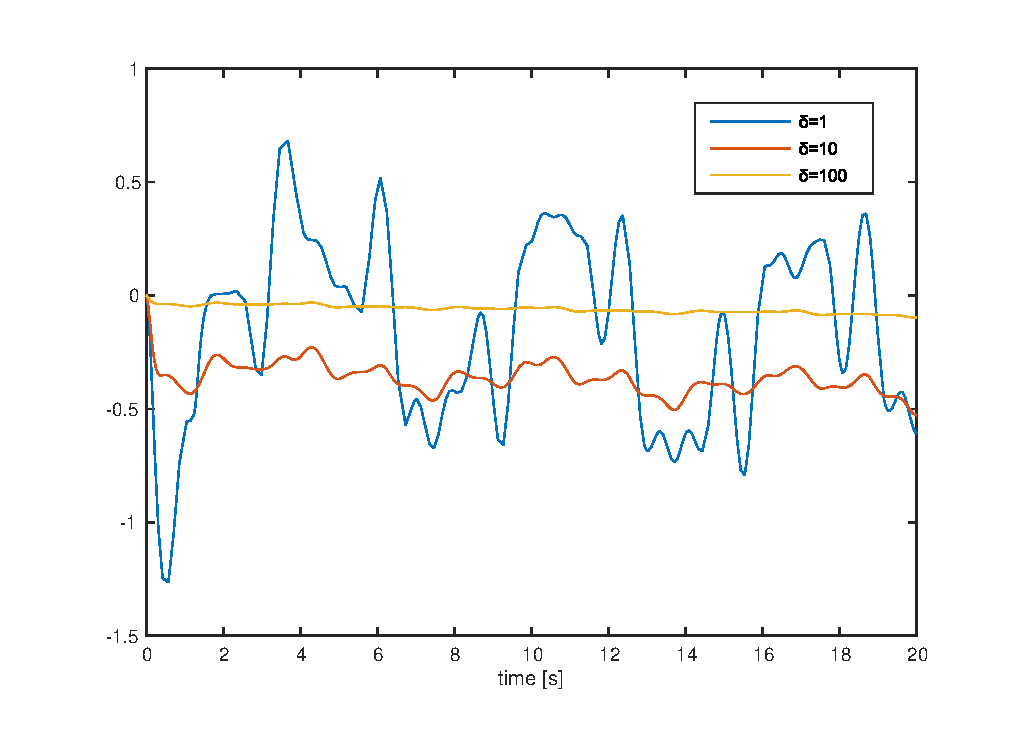
\includegraphics[width=85mm]{fig/gamma_h_rdsin.eps}
        \caption{$r_d(t)=4+0.5\sin 0.5t + \cos 3t - 2\sin 5t$のときの$\hat{\gamma}$($\delta=1,10,100$)の様子}
        \label{fig:gamma_h_rdsin}
    \end{center}
\end{figure}
%
%%%%%%%%%%%%%%%%%%%%%%%%%%%%
\section{考察}
%%%%%%%%%%%%%%%%%%%%%%%%%%%%
図\ref{fig:x_rd4},\ref{fig:x_rdsin}を見ると設計パラメータ$\delta$を大き
くすればするほど,理想軌道に対する追従性能が向上していることがわかる.し
かし,大きくし過ぎると追従性能は向上しているが,小さく振動していることが確認で
きた.次に,$\delta=10$とし,$\eta_\alpha,\eta_\beta,\eta_\gamma$のうちひ
とつだけ値を変化させたときの応答を図\ref{fig:x_rd4etaa} -
\ref{fig:x_rd4etag2}示す.ただし,$r_d(t)=4$とした.図\ref{fig:x_rd4etaa}より$\eta_\alpha$を増加させると追従性能が向上するこ
とがわかる.また,図\ref{fig:x_rd4etab}より,$\eta_\beta$を増加させると,
応答が発散することがわかった.最後に,図
\ref{fig:x_rd4etag},\ref{fig:x_rd4etag2}より,$\eta_\gamma$を増加させる
と定常状態においての追従性能は変わらなかったが,過渡状態(特に時間$t=0〜1$[s])
において,$\eta_\gamma$が増加すると追従性能が上がることがわかった.最後
に,$\eta_\alpha=1000,\eta_\beta=\eta_\alpha=1000,\eta_\gamma=\eta^\frac{3}{2}_\alpha=31622$とした場合と,
$\eta_\alpha=1,\eta_\beta=1,\eta_\gamma=1$としたときの比較をしたものを図
\ref{fig:x_rd4_eta_reform}に示す.ただし,$\delta=10$とした.図\ref{fig:x_rd4_eta_reform}を見ると,
推定ゲイン$\eta$を調整することでより良い制御性能が得られることがわかった.また,$\eta$を変化させたときの$u(t)$を比較したものを図
\ref{fig:eta_hikaku},\ref{fig:eta_hikaku_k}に示す.$\eta$を大きくすると
良い制御性能を得られることがわかったが図
\ref{fig:eta_hikaku},\ref{fig:eta_hikaku_k}を見ると,$\eta$を大きくする
と$u(t)$が時間$0〜0.3$[s]において振動することがわかった.
\\

%
\begin{figure}[tb]
    \begin{center}
       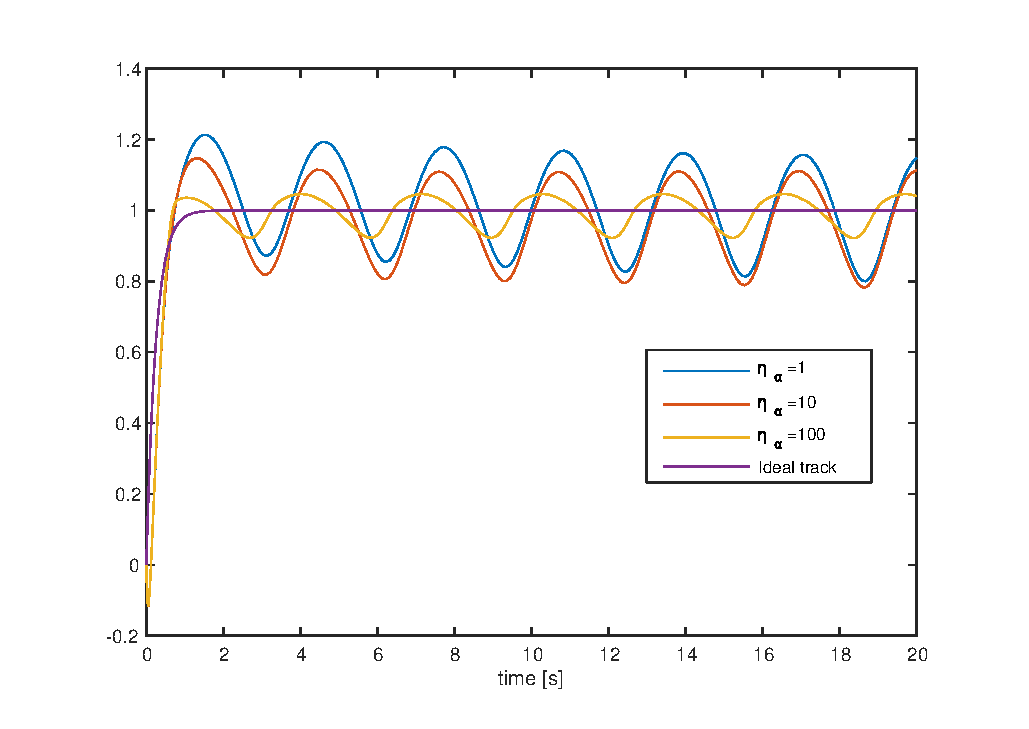
\includegraphics[width=140mm]{fig/x_rd4_Etaa.eps}
        \caption{$\eta_\alpha$を変化させたとき$x(t)$の様子($r_d(t)=4$の
	 とき)}
        \label{fig:x_rd4etaa}
    \end{center}
\end{figure}
%
%
\begin{figure}[ht]
    \begin{center}
       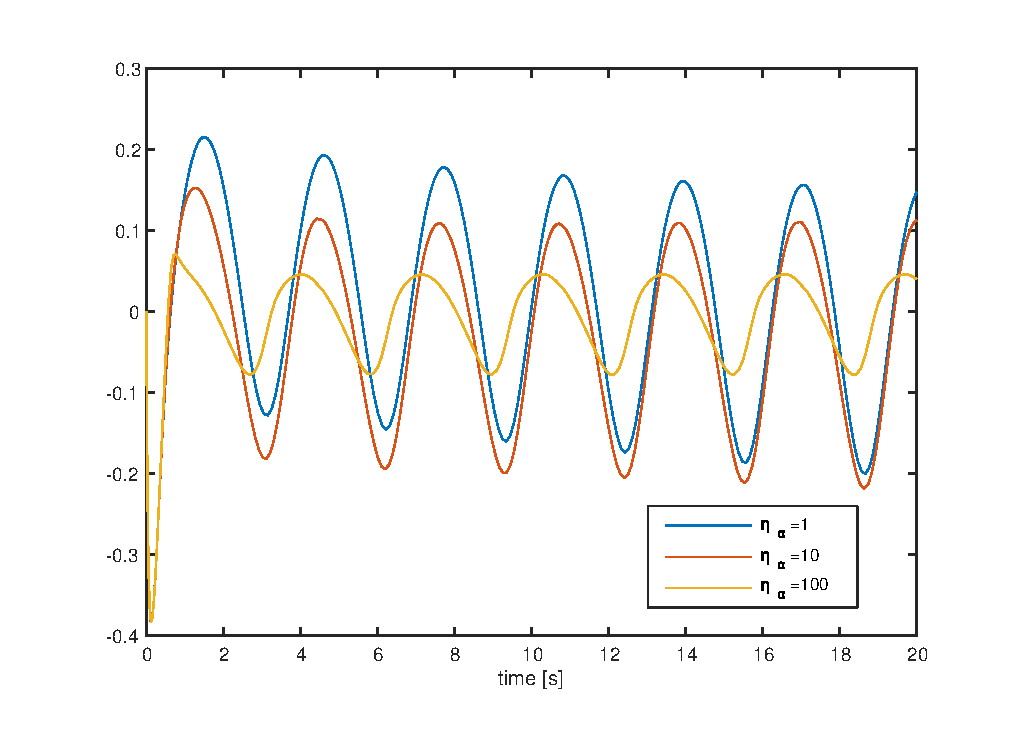
\includegraphics[width=140mm]{fig/x_tilde_etaa.eps}
        \caption{$\eta_\alpha$を変化させたときの$\tilde{x}(t)$の様子($r_d(t)=4$の
	 とき)}
        \label{fig:x_tilde_etaa}
    \end{center}
\end{figure}
%
%
\begin{figure}[htb]
    \begin{center}
       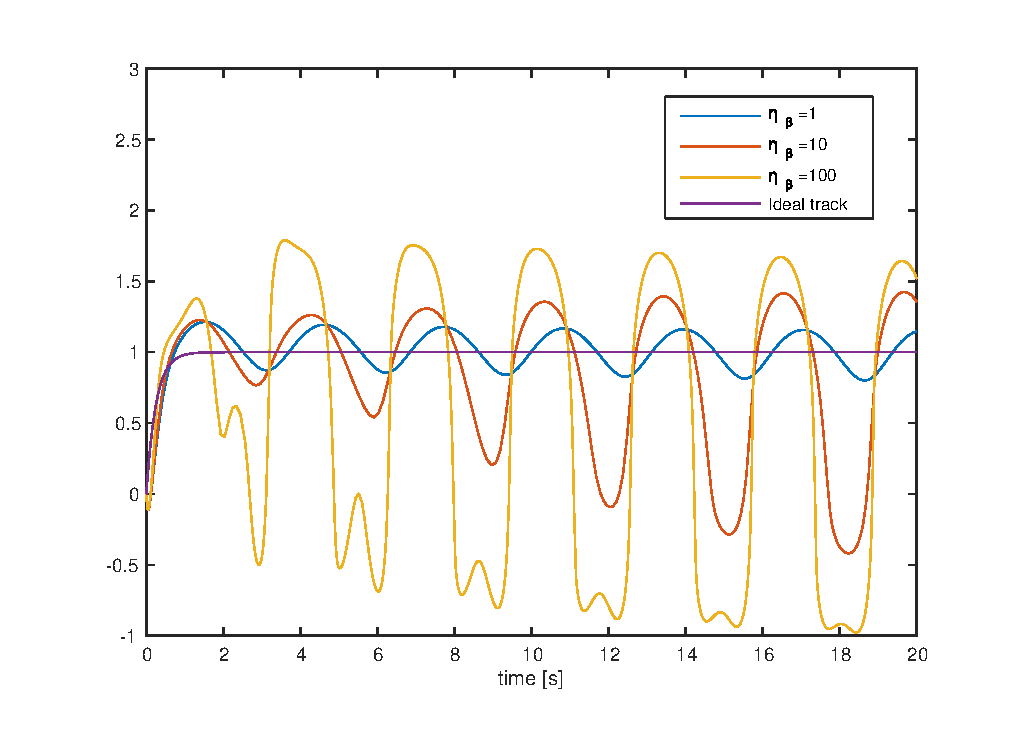
\includegraphics[width=140mm]{fig/x_rd4_Etab.eps}
        \caption{$\eta_\beta$を変化させたときの$x(t)$の様子($r_d(t)=4$のとき)}
        \label{fig:x_rd4etab}
    \end{center}
\end{figure}
%
%
\begin{figure}[htb]
    \begin{center}
       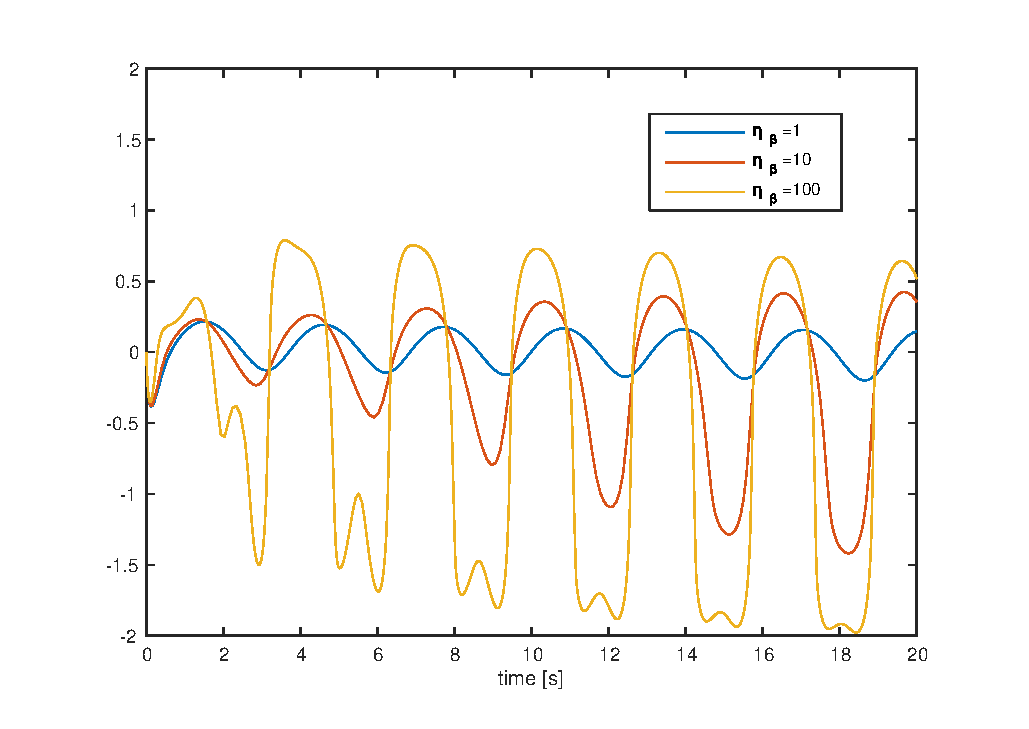
\includegraphics[width=140mm]{fig/x_tilde_etab.eps}
        \caption{$\eta_\beta$を変化させたときの$\tilde{x}(t)$の様子($r_d(t)=4$のとき)}
        \label{fig:x_tilde_etab}
    \end{center}
\end{figure}
%
%
\begin{figure}[htb]
    \begin{center}
       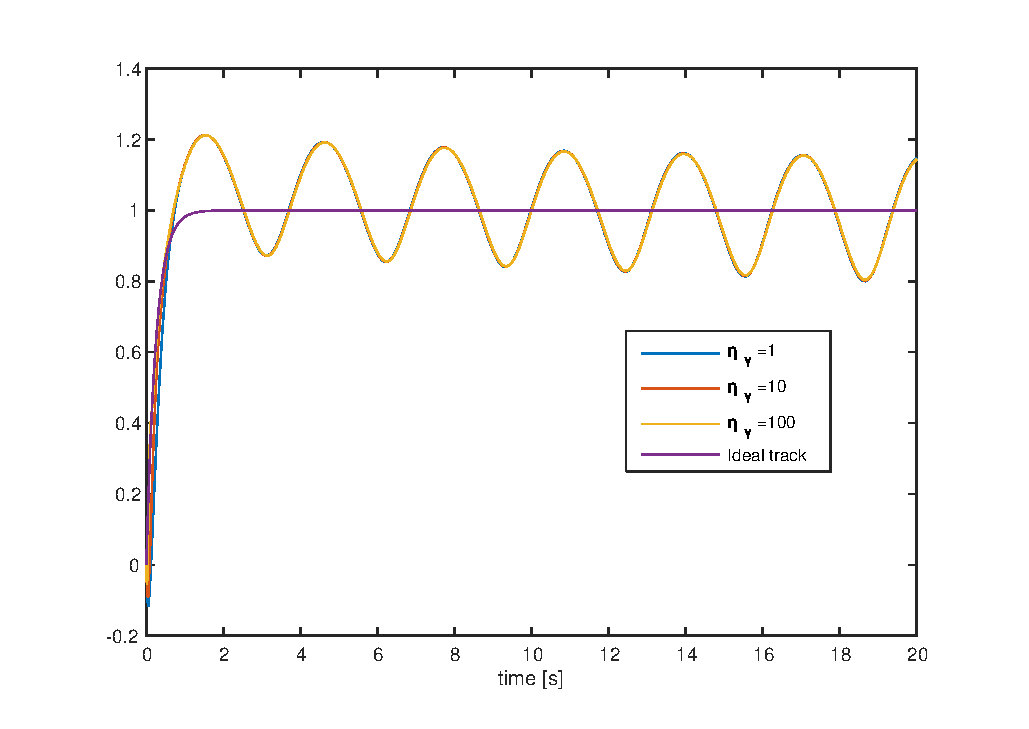
\includegraphics[width=140mm]{fig/x_rd4_Etag.eps}
	 \caption{$\eta_\gamma$を変化させたときの$x(t)$の様子$r_d(t)=4$のとき)
	 }
        \label{fig:x_rd4etag}
    \end{center}
\end{figure}
%
%
\begin{figure}[htb]
    \begin{center}
       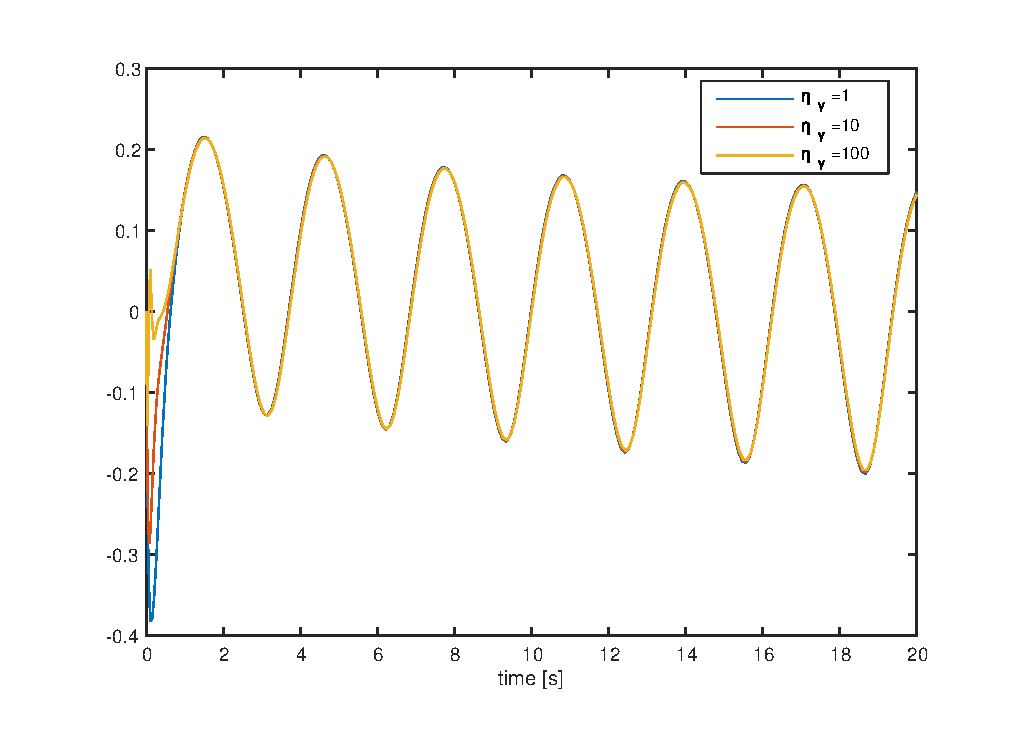
\includegraphics[width=140mm]{fig/x_tilde_etag.eps}
	 \caption{$\eta_\gamma$を変化させたときの$\tilde{x}(t)$の様子($r_d(t)=4$のとき)
	 }
        \label{fig:x_tilde_etag}
    \end{center}
\end{figure}
%
%
\begin{figure}[p]
    \begin{center}
	 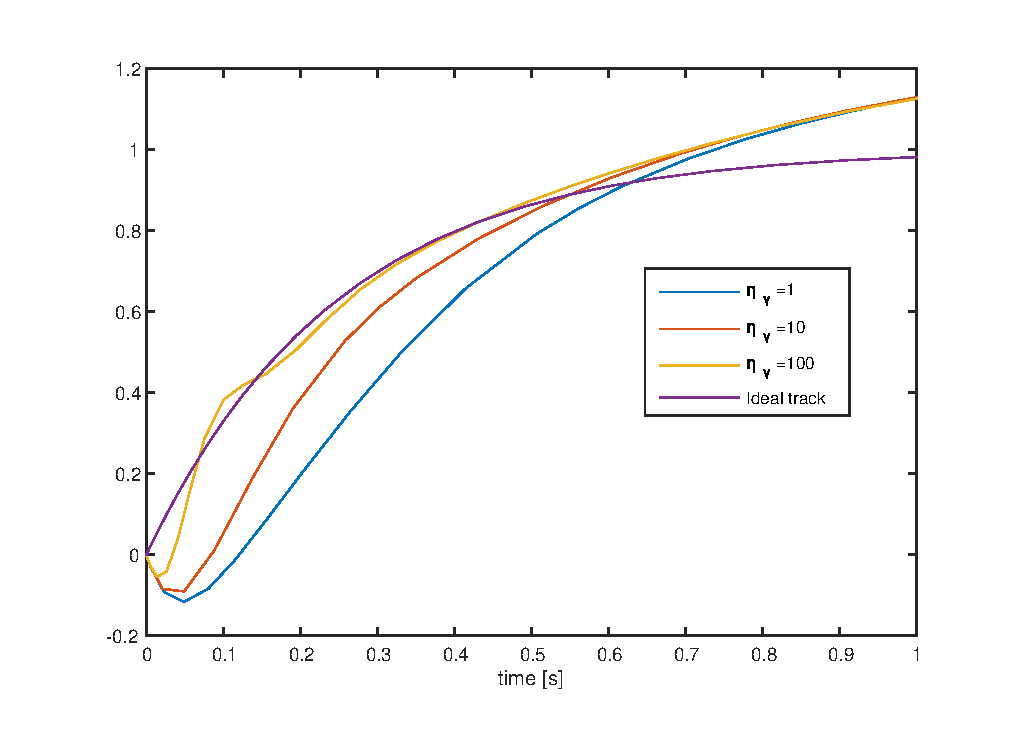
\includegraphics[width=180mm]{fig/x_rd4_Etag_2.eps}
        \caption{図\ref{fig:x_rd4etag}の拡大図(時間$t=0〜1$[s]について)}
        \label{fig:x_rd4etag2}
    \end{center}
\end{figure}
%
%
\begin{figure}[htb]
    \begin{center}
	 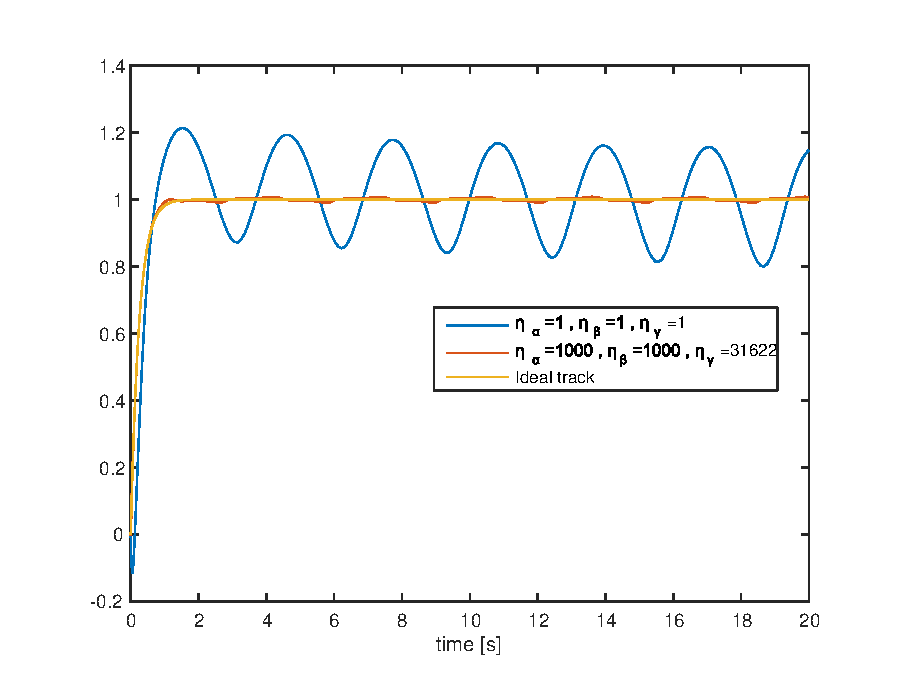
\includegraphics[width=140mm]{fig/x_rd4_eta_reform.eps}
	 \caption{$\eta_\alpha,\eta_\beta,\eta_\gamma$を変化させたときの$x(t)$の様子}
        \label{fig:x_rd4_eta_reform}
    \end{center}
\end{figure}
%
%
\begin{figure}[htb]
    \begin{center}
	 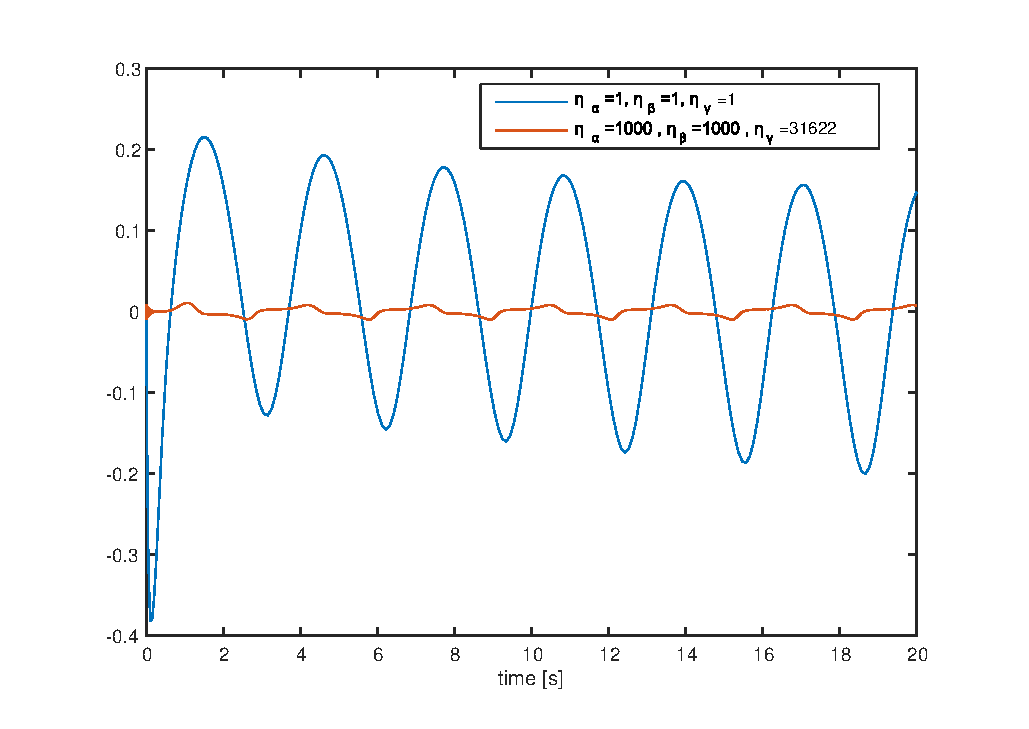
\includegraphics[width=140mm]{fig/x_tilde_eta_all.eps}
	 \caption{$\eta_\alpha,\eta_\beta,\eta_\gamma$を変化させたときの$\tilde{x}(t)$の様子}
        \label{fig:x_tilde_eta_all}
    \end{center}
\end{figure}
%
%
\begin{figure}[htb]
    \begin{center}
	 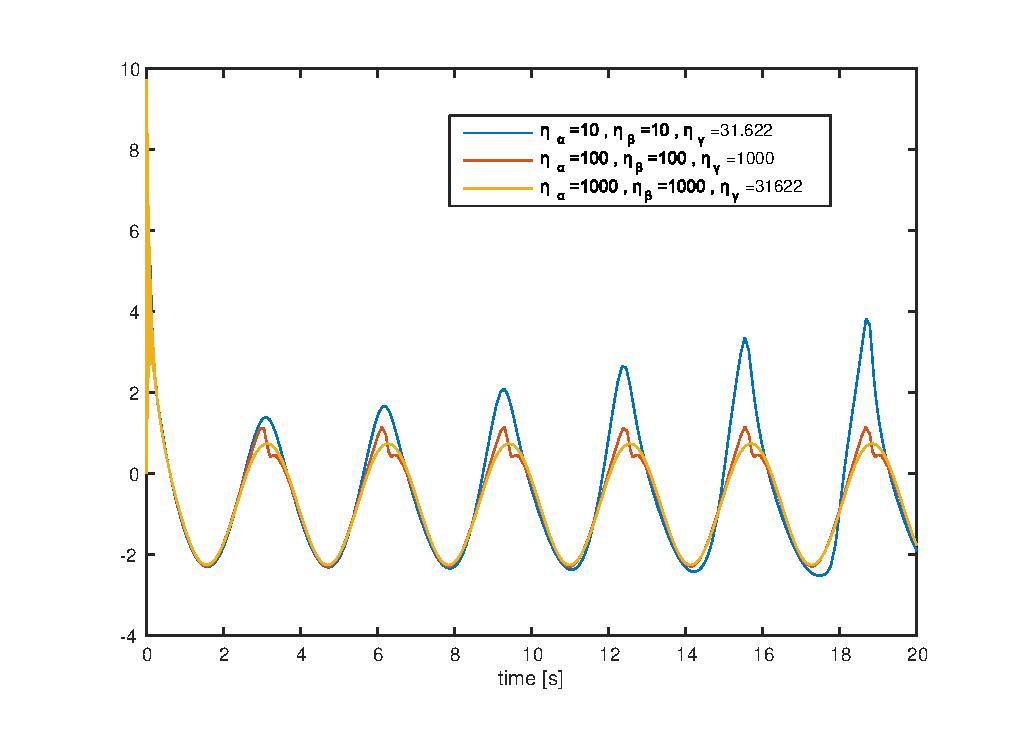
\includegraphics[width=140mm]{fig/eta_hikaku.eps}
        \caption{$\eta_\alpha,\eta_\beta,\eta_\gamma$を変化させたときの$u(t)$の様子}
        \label{fig:eta_hikaku}
    \end{center}
\end{figure}
%
%
\begin{figure}[htb]
    \begin{center}
	 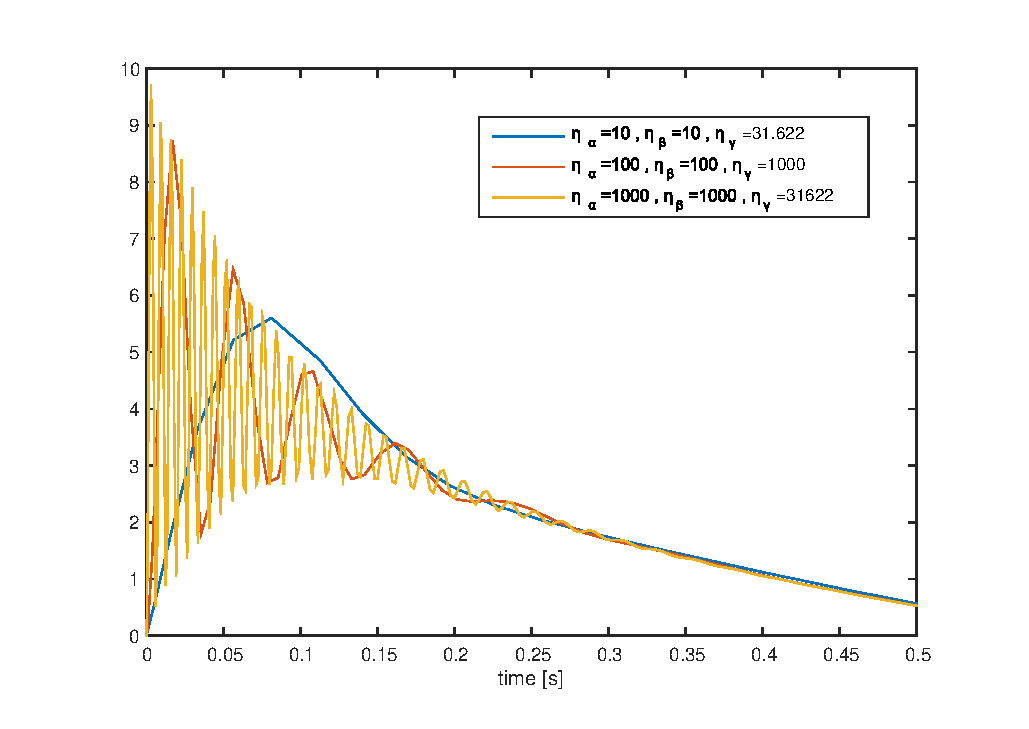
\includegraphics[width=140mm]{fig/eta_hikaku_k.eps}
        \caption{図\ref{fig:eta_hikaku}の拡大図}
        \label{fig:eta_hikaku_k}
    \end{center}
\end{figure}
%
%
%
%
\clearpage

\begin{thebibliography}{99}
 \addcontentsline{toc}{section}{参考文献}

 \bibitem{jamming} 大屋勝敬:"車両制御特論MATLAB+Simulinkの利用法"
\end{thebibliography}

\end{document}
